\documentclass[11pt,letterpaper]{article}
\PassOptionsToPackage{hyphens}{url}
\usepackage[margin=.83in,top=.8in,bottom=.8in,headheight=15pt]{geometry}
\usepackage[T1]{fontenc}
\usepackage{lmodern,amsmath,amssymb,mathtools,bm,booktabs,array,graphicx,tikz}
\usetikzlibrary{arrows.meta,positioning,calc,decorations.pathreplacing,patterns}
\definecolor{ink}{HTML}{17344D}\definecolor{accent}{HTML}{087E8B}\definecolor{pale}{HTML}{EDF5F5}\definecolor{gold}{HTML}{AD6B19}
\providecommand{\dd}{\,\mathrm{d}}\providecommand{\R}{\mathbb{R}}
\providecommand{\E}{\mathbb{E}}\providecommand{\Var}{\operatorname{Var}}
\providecommand{\Cov}{\operatorname{Cov}}\providecommand{\diag}{\operatorname{diag}}
\providecommand{\norm}[1]{\left\lVert#1\right\rVert}
\providecommand{\abs}[1]{\left|#1\right|}
\usepackage{microtype,hyperref,fancyhdr,enumitem,amsthm,sectsty,needspace}
\allsectionsfont{\raggedright}
\hypersetup{colorlinks=true,linkcolor=ink,urlcolor=accent,pdfauthor={Zan Ahmad},pdftitle={Cable equations and propagation through a branch / Lecture notes}}
\setlength{\parindent}{0pt}\setlength{\parskip}{6pt}\linespread{1.07}
\setlist{itemsep=3pt,topsep=4pt,leftmargin=*}
\emergencystretch=2em\clubpenalty=10000\widowpenalty=10000
\pagestyle{fancy}\fancyhf{}\fancyhead[L]{\small Mathematical Modeling}\fancyhead[R]{\small Lecture 10}
\fancyfoot[L]{\footnotesize Zan Ahmad}\fancyfoot[R]{\footnotesize\thepage}\renewcommand{\headrulewidth}{.3pt}
\newtheorem{proposition}{Proposition}\newtheorem{theorem}{Theorem}\newtheorem{lemma}{Lemma}
\theoremstyle{definition}\newtheorem{definition}{Definition}\newtheorem{example}{Example}
\numberwithin{equation}{section}
\begin{document}
{\small\scshape Mathematical Modeling\hfill Lecture 10}\par\medskip
{\raggedright\hyphenpenalty=10000\exhyphenpenalty=10000\LARGE\bfseries\color{ink} Cable equations and propagation through a branch\par}\medskip
{\small Lecture notes}\par\bigskip
A spatial membrane model combines axial Ohm law, local charge storage, and voltage-dependent ionic currents. We derive the continuous cable equation, construct a conservative network discretization, and analyze the coupled voltage solve before interpreting the branched neuronal experiment.

\section{Axial conduction and local charge conservation}
\hypertarget{note-axial-conduction-and-local-charge-conservation}{}\label{note:axial-conduction-and-local-charge-conservation}
{\small \href{slides.html\#frame=axial-ohm-law\&step=1}{Slides for this section}}\par
Let $V(x,t)$ be membrane voltage along a cylindrical cable of radius $a$. Assume the extracellular potential is spatially uniform, so the axial gradient of intracellular potential equals $\partial_xV$. For intracellular resistivity $\rho$, Ohm's law gives total axial current in the positive $x$ direction:
\[
I_a=-\frac{\pi a^2}{\rho}\,\partial_xV.
\]
For a segment $[x,x+\Delta x]$, axial inflow minus outflow charges the membrane and supplies its outward ionic current. Dividing by length and taking the limit gives
\[
-\partial_x I_a=2\pi a(C\partial_tV+I_{\mathrm{ion}}-I_{\mathrm{app}}).
\]
Here $C$ is capacitance per membrane area and the two membrane currents are densities. With constant radius and resistivity,
\[
\boxed{C\partial_tV=\frac a{2\rho}\partial_{xx}V-I_{\mathrm{ion}}+I_{\mathrm{app}}.}
\]
This is a reaction--diffusion cable equation, not the second-order-in-time wave equation. Traveling spikes arise from axial conduction coupled to local nonlinear ionic feedback. The derivation would change if an extracellular voltage gradient contributed appreciably.
\section{Passive length and time scales}
\hypertarget{note-passive-length-and-time-scales}{}\label{note:passive-length-and-time-scales}
{\small \href{slides.html\#frame=passive-membrane-scales\&step=1}{Slides for this section}}\par
For a passive membrane with $I_{\mathrm{ion}}=g_L(V-E_L)$ and no applied current, put $u=V-E_L$. Then
\[
\tau_m\partial_tu=\lambda^2\partial_{xx}u-u,\qquad
\tau_m=\frac C{g_L},\quad \lambda^2=\frac a{2\rho g_L}.
\]
The time constant describes local capacitive relaxation; the length constant describes steady spatial attenuation. On a semi-infinite cable, a bounded steady solution with specified endpoint voltage decays as $e^{-x/\lambda}$. That profile is not itself a propagating action potential.

On a sealed interval of length $\ell$, $\partial_xu=0$ at both ends. A cosine mode has the exact solution
\[
u(x,t)=B\cos(kx)\exp\left[-\left(Dk^2+g_L/C\right)t\right],
\quad k=j\pi/\ell,\quad D=\frac a{2\rho C}.
\]
This provides a verification benchmark without active gates. It separates the spatial operator from the nonlinear membrane mechanisms. A passive disturbance spreads and decays; an active spike can be regenerated by the channel dynamics in neighboring regions.
\section{A conservative network discretization}
\hypertarget{note-a-conservative-network-discretization}{}\label{note:a-conservative-network-discretization}
{\small \href{slides.html\#frame=shared-edge-currents\&step=1}{Slides for this section}}\par
For an edge of radius $r_{ij}$ and length $\Delta x_{ij}$, define
\[
K_{ij}=\frac{\pi r_{ij}^2}{\rho\Delta x_{ij}},\qquad
I_{i\to j}=K_{ij}(V_i-V_j).
\]
The same edge current enters node $j$ with the opposite sign. In the companion, lengths and radii are in centimeters and $\rho=0.0354\,\mathrm{k}\Omega\,\mathrm{cm}$, so $K$ is in millisiemens and $I_{i\to j}$ is in microamperes. It is a total current, not a membrane current density.

Assign half the cylindrical lateral area of each edge to each endpoint:
\[
A_i=\sum_{j\sim i}\pi r_{ij}\Delta x_{ij},\qquad M_i=CA_i.
\]
Thus $\sum_iA_i=\sum_{\{i,j\}}2\pi r_{ij}\Delta x_{ij}$. End caps and a separate soma are not included. The finite-volume node equation is
\[
\boxed{M_i\dot V_i+A_iI_{\mathrm{ion},i}
+\sum_{j\sim i}K_{ij}(V_i-V_j)=I_{\mathrm{app},i}.}
\]
Every term is a total current. A terminal node has half an edge's lateral area; an interior node receives contributions from two edges; a branch node receives one from each incident edge. A shared junction has one voltage, not three disconnected copies.
\section{Junction storage and the summed current budget}
\hypertarget{note-junction-storage-and-the-summed-current-budget}{}\label{note:junction-storage-and-the-summed-current-budget}
{\small \href{slides.html\#frame=a-charging-branch-junction\&step=1}{Slides for this section}}\par
A branch node may simultaneously receive axial current, send current into daughters, carry membrane current, and charge. For trunk inflow $0.006\,\mu\mathrm A$, daughter outflows $0.002$ and $0.001\,\mu\mathrm A$, and outward ionic current $0.001\,\mu\mathrm A$, the capacitive remainder is
\[
I_C=0.006-0.002-0.001-0.001=0.002\,\mu\mathrm A.
\]
For node capacitance $0.0002\,\mu\mathrm F$, $\dot V=10\,\mathrm{mV/ms}$, giving an initial $0.1\,\mathrm{mV}$ rise over $0.01\,\mathrm{ms}$. Daughter currents need not sum to trunk current while the finite junction membrane stores charge and carries ionic current. A zero-volume continuum junction has a different limiting balance.

Define the symmetric graph Laplacian by $(LV)_i=\sum_jK_{ij}(V_i-V_j)$. Its rows sum to zero, so adding all node equations cancels axial currents:
\[
\frac{\dd}{\dd t}\sum_iM_iV_i+\sum_iA_iI_{\mathrm{ion},i}
=\sum_iI_{\mathrm{app},i}.
\]
With constant capacitances, $\sum_iM_iV_i$ is the stored-charge variable in this model. The unweighted sum of voltages is not the conserved quantity. Even weighted charge changes when ionic or applied membrane currents are present. Sealed ends prohibit external axial current; they do not turn off transmembrane ionic current.
\section{The coupled implicit voltage solve}
\hypertarget{note-the-coupled-implicit-voltage-solve}{}\label{note:the-coupled-implicit-voltage-solve}
{\small \href{slides.html\#frame=the-graph-laplacian\&step=1}{Slides for this section}}\par
The teaching solver first updates gates exactly with rates frozen at the old local voltages. Denote the resulting conductance densities by $g_{ij}^{k+1}$, where $j$ indexes ionic channel types. Set
\[
G_i=\sum_jg_{ij}^{k+1},\quad b_i=\sum_jg_{ij}^{k+1}E_j,\quad
M=\operatorname{diag}(M_i),\quad D_A=\operatorname{diag}(A_i).
\]
A backward-Euler voltage balance with these frozen conductances is
\[
\left(\frac M{\Delta t}+L+D_A\operatorname{diag}(G)\right)V^{k+1}
=\frac M{\Delta t}V^k+D_Ab+I_{\mathrm{app}}.
\]
This solves all new voltages simultaneously, including the axial coupling. It is not the single-cell exponential voltage step used in the preceding lesson, and it is not the source report's staggered Crank--Nicolson scheme.

For any nonzero vector $z$,
\[
z^TLz=\sum_{\{i,j\}}K_{ij}(z_i-z_j)^2\geq0.
\]
Because $M_i>0$ and $\Delta t>0$, the full matrix is symmetric positive definite. The tree solver eliminates leaves toward the root and then back-substitutes. Eliminating a leaf $i$ with diagonal $d_i$ and parent $p$ changes the parent's diagonal and right side by
\[
d_p\leftarrow d_p-K_{ip}^2/d_i,\qquad
r_p\leftarrow r_p+K_{ip}r_i/d_i.
\]
This is ordinary elimination specialized to the tree sparsity, not an approximation to the matrix solve. Time discretization and spatial discretization remain separate approximations.
\section{A branched neuronal experiment}
\hypertarget{note-a-branched-neuronal-experiment}{}\label{note:a-branched-neuronal-experiment}
{\small \href{slides.html\#frame=the-synthetic-branched-experiment-figure\&step=1}{Slides for this section}}\par
The synthetic geometry has a $3\,\mathrm{mm}$ trunk and two $2\,\mathrm{mm}$ daughters. Trunk and upper-daughter radii are $5\,\mu\mathrm m$; lower radius is $3.5\,\mu\mathrm m$. Thirty trunk intervals and twenty per daughter yield $71$ shared nodes. The angle in the drawing indicates connectivity; physical edge lengths determine the conductances and areas.

All nodes start from the computed neuronal resting state. A total current $0.006\,\mu\mathrm A$ is applied at the start from $1$ to $2\,\mathrm{ms}$, delivering $0.006\,\mu\mathrm A\,\mathrm{ms}$. With nominal step $0.005\,\mathrm{ms}$, the first upward zero crossings occur near $2.189$, $3.799$, $4.692$, and $4.913\,\mathrm{ms}$ at the start, junction, upper tip, and lower tip. The thinner daughter is later in this experiment; no universal propagation rule follows from one geometry.

A time trace fixes location, while a spatial snapshot fixes time. The snapshots at $2.5$, $3.5$, and $4.5\,\mathrm{ms}$ share the same trunk in both path panels because they come from one coupled network. The local channel response regenerates voltage as axial current reaches adjacent regions; the plot does not track a single packet of sodium ions traveling from start to tip.
\begin{center}\begin{minipage}{.98\linewidth}\centering
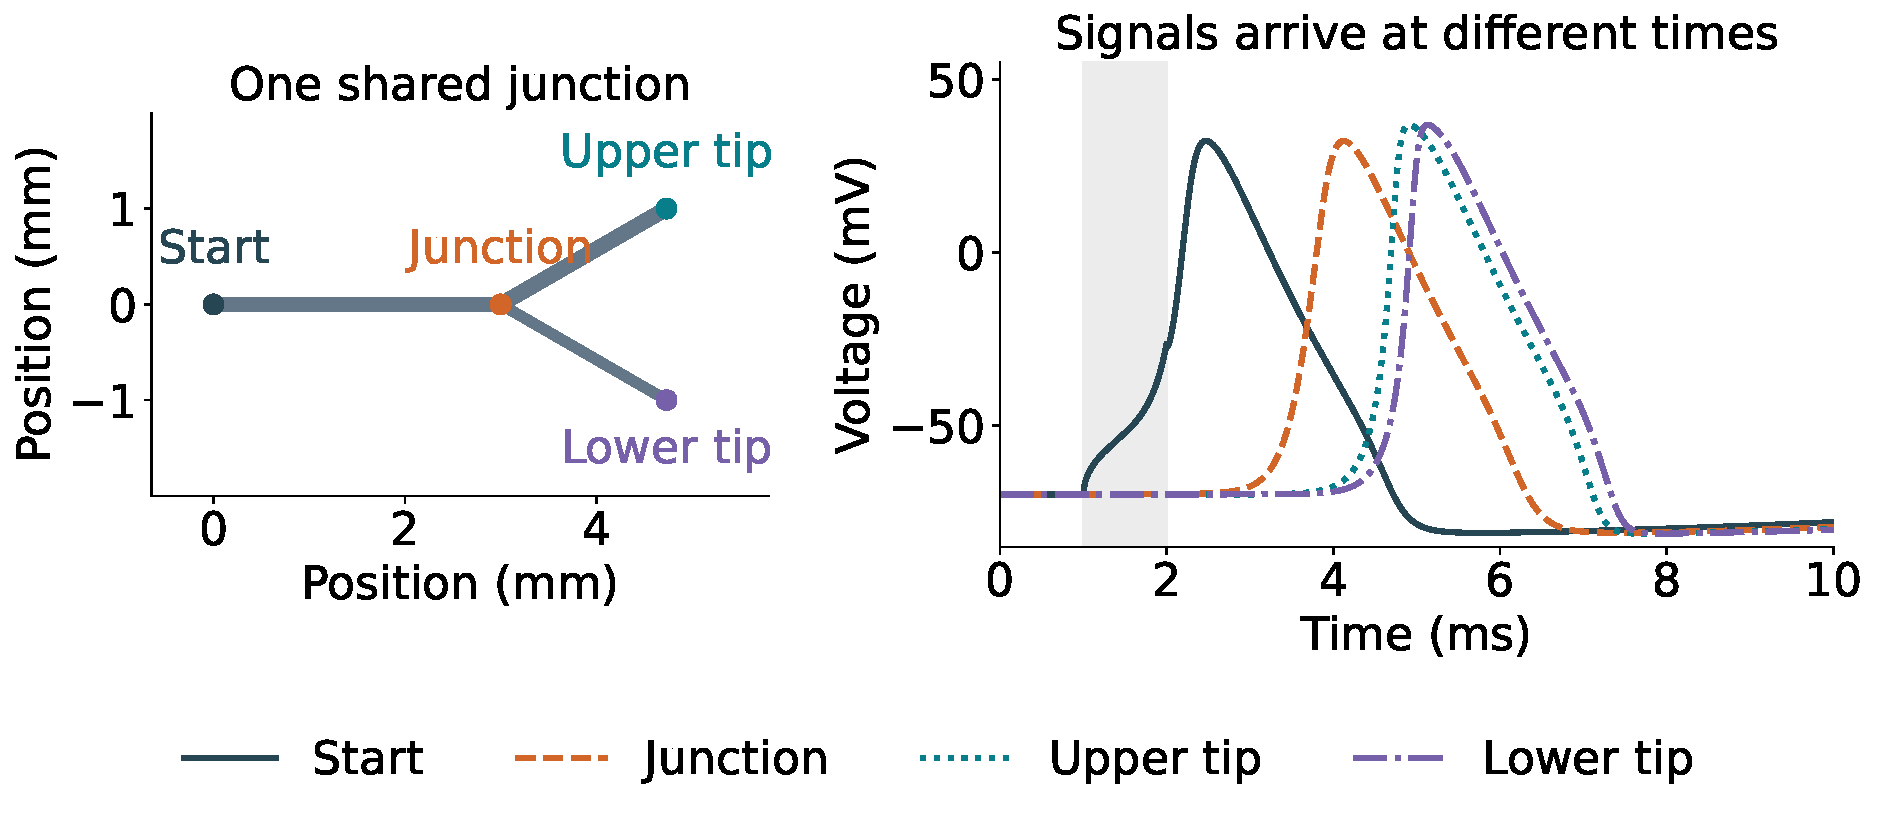
\includegraphics[width=.96\linewidth,height=.57\textheight,keepaspectratio]{branched-probes.pdf}\par\smallskip
{\small Synthetic neuronal cable with a 3 mm trunk and two 2 mm daughters. Trunk/upper radii 5 $\mu$m; lower radius 3.5 $\mu$m. Total input 0.006 $\mu$A from 1 to 2 ms (gray band), nominal step 0.005 ms. These are computed local voltages.}
\end{minipage}\end{center}
\section{Arrival measurements and independent numerical checks}
\hypertarget{note-arrival-measurements-and-independent-numerical-checks}{}\label{note:arrival-measurements-and-independent-numerical-checks}
{\small \href{slides.html\#frame=threshold-based-arrival-and-speed\&step=1}{Slides for this section}}\par
Define an arrival by the first upward crossing of a stated threshold. The companion linearly interpolates between the two stored values that bracket $0\,\mathrm{mV}$. For two probes separated by physical path length $d$, the event-based average speed is $d/(t_2-t_1)$. The upper daughter gives approximately $2\,\mathrm{mm}/0.893\,\mathrm{ms}=2.24\,\mathrm{m/s}$. Dividing by time since stimulus onset would include initiation delay and answer a different question.

The companion verifies tree elimination against dense matrix solves on small trees, sums node areas against the cylindrical lateral area, checks stationary rest and equal-daughter symmetry, and audits the fully discrete current budget
\[
\sum_iM_i(V_i^{k+1}-V_i^k)
+\Delta t\sum_i A_i(G_iV_i^{k+1}-b_i)
-\Delta t\sum_iI_{\mathrm{app},i}=0.
\]
This residual uses the actual frozen conductances and new voltages of the scheme. An unrelated continuous-time quadrature would test a different identity.

The passive cosine benchmark isolates spatial error, with approximately second-order refinement in the verified setup. Exact evolution of the same spatially discrete linear system isolates the first-order time error of backward Euler. Active tip-arrival differences decrease under time-step refinement at the fixed mesh; this does not complete an active spatial-convergence study. For biological validation one would additionally need measured geometry, stimulus, recording locations, environmental conditions, and independent waveforms. Fixed reversal potentials and omitted extracellular gradients are substantive model assumptions.
\begin{center}\begin{minipage}{.98\linewidth}\centering
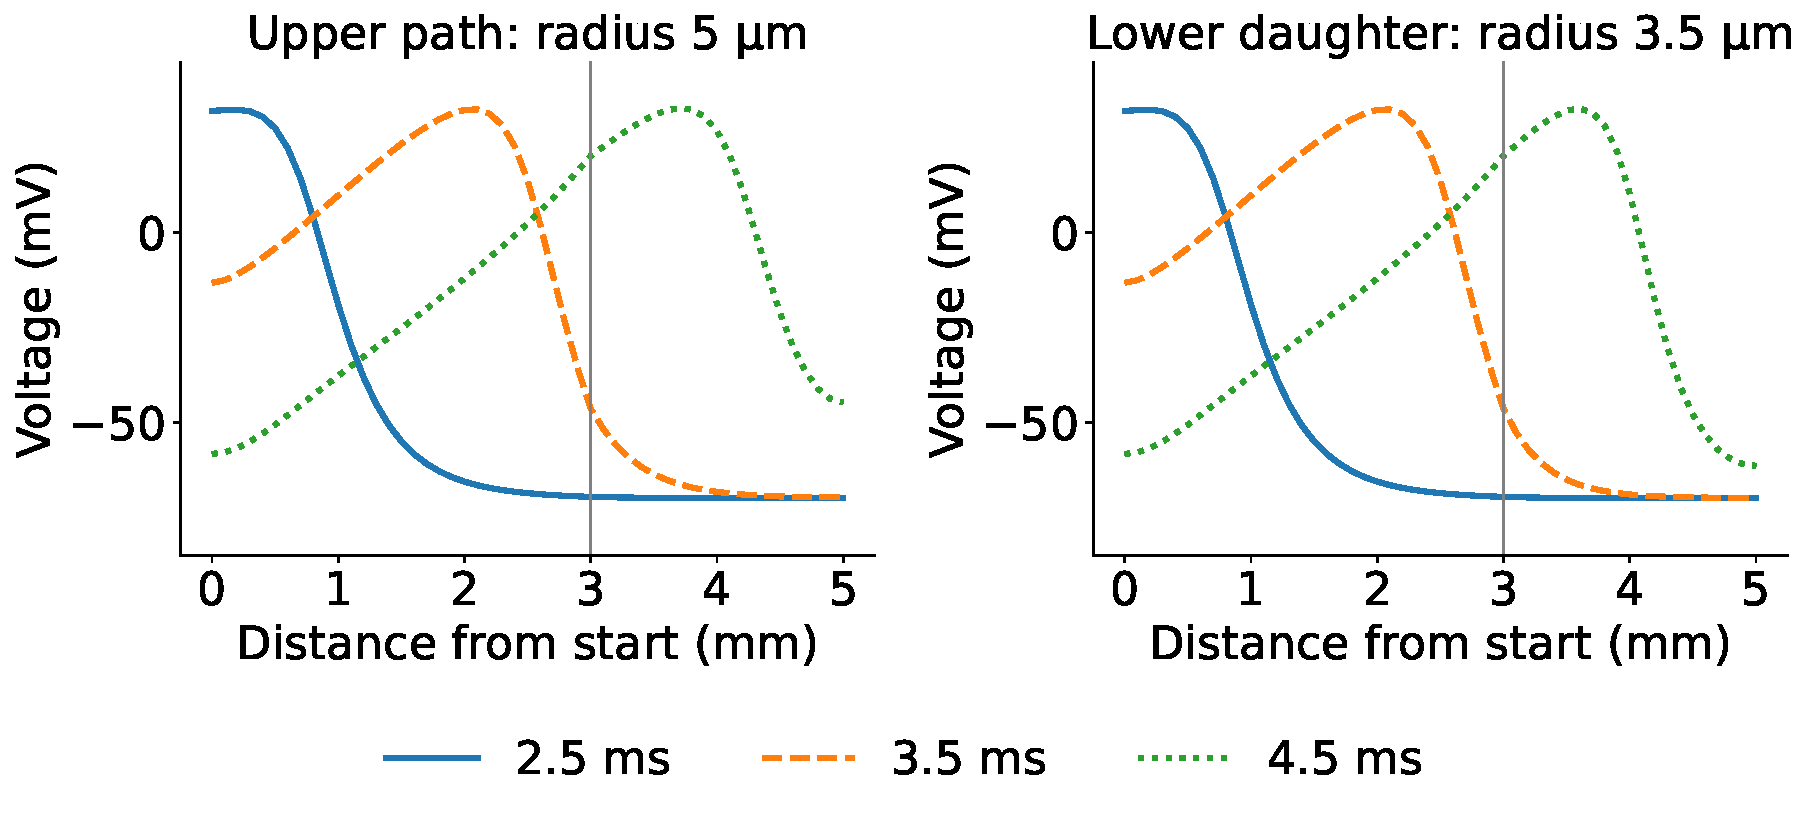
\includegraphics[width=.96\linewidth,height=.57\textheight,keepaspectratio]{traveling-profiles.pdf}\par\smallskip
{\small Three snapshots from the same coupled experiment, plotted along the upper and lower paths. The junction lies at path distance 3 mm (vertical line). Only the lower daughter narrows; both panels share the same trunk.}
\end{minipage}\end{center}
\bigskip
\section*{Exercises}
\par\noindent\begin{minipage}{\linewidth}
\subsection*{MM10-E1. Account for a shared junction}
A different junction state receives 0.005 $\mu$A from its trunk. Daughter outflows are 0.003 and 0.001 $\mu$A. Ionic outflow is 0.002 $\mu$A and total capacitance 0.0002 $\mu$F.

\textbf{a} Find net capacitive current and its sign.

\end{minipage}\par\medskip
\textbf{b} Estimate the signed voltage change over 0.02 ms using the starting rate. Does voltage rise or fall?

\textbf{c} Why is requiring the two daughter currents to sum to trunk current incorrect here?

\par\noindent\begin{minipage}{\linewidth}
\subsection*{MM10-E2. Read an arrival-time measurement}
Two probes 2 mm apart along one daughter first cross upward through 0 mV at 3.80 and 4.70 ms.

\textbf{a} Find propagation delay and average speed between them.

\end{minipage}\par\medskip
\textbf{b} If stimulus onset was 1 ms, why is 2/(4.70 - 1) a different quantity?

\textbf{c} What must be reported if a tip never crosses the chosen threshold?

\par\noindent\begin{minipage}{\linewidth}
\subsection*{MM10-E3. Change geometry and track units}
A cylindrical segment has axial conductance K =\allowbreak{} pi r$^2$/(rho length) and lateral membrane area A =\allowbreak{} 2 pi r length.

\textbf{a} At fixed length and resistivity, how do K and A change when radius doubles?

\end{minipage}\par\medskip
\textbf{b} At fixed radius, what happens to each when length is halved?

\textbf{c} Why cannot one infer an exact doubling of active propagation speed solely from the first calculation?

\par\noindent\begin{minipage}{\linewidth}
\subsection*{MM10-E4. Audit a conservation claim}
A student says: ``My branch model has a smooth wave and exactly conserved internal axial current, so it is accurate and predicts actual neurons.''

\textbf{a} What does internal current cancellation test?

\end{minipage}\par\medskip
\textbf{b} Give a numerical accuracy test using time refinement or a suitable reference, and state the spatial error that a fixed-mesh time test leaves unresolved.

\textbf{c} Give a separate test of biological interpretation and one missing mechanism.

\section*{References}
\noindent\begin{minipage}{\linewidth}
Zan Ahmad, Fall 2024 HEART syllabus. PDF pages 1--2.

\end{minipage}\par\medskip
\noindent\begin{minipage}{\linewidth}
Zan Ahmad, Action Potential Propagation in Branched Neuronal Cables. Current report, PDF pages 1--4.

\url{https://zanahmad.com/files/AP_Propagation.pdf}
\end{minipage}\par\medskip
\noindent\begin{minipage}{\linewidth}
Hoppensteadt and Peskin, Modeling and Simulation in Medicine and the Life Sciences, second edition. Printed page 126 and pages 313--317; supplied PDF page 139 and pages 323--327.

\end{minipage}\par\medskip
\end{document}
